\documentclass{report}
\usepackage{graphicx} % Required for inserting images
\usepackage[italian]{babel}
\usepackage{tikz}
\usepackage{hyperref}
\usepackage{amsmath}
\usepackage{xcolor}
\usepackage{float}
\usepackage{soul}
\usepackage{listings} % Per evidenziare il codice

\definecolor{lightgray}{rgb}{0.9,0.9,0.9} % Definizione colore sfondo
\definecolor{darkgreen}{rgb}{0.0, 0.5, 0.0}

\lstset{
    backgroundcolor=\color{lightgray}, % Sfondo grigio
    basicstyle=\ttfamily, % Font monospaziato
    % frame=single, % Bordo attorno al codice
    tabsize=4, % Dimensione tabulazione
    breaklines=true, % Permette di andare a capo automaticamente
    numbers = left,
    numberstyle=\small\color{gray}
}

\title{\huge\textbf{{Refresher}}}
\date{Parte I}

\begin{document}

\maketitle
\tableofcontents
\newpage


\chapter{Basics}

\section{Introduzione al decision making}

Il \textit{decision making} è una parte integrante del ruolo di gestione; i dirigenti prendono centinaia di decisioni ogni giorno.

\noindent La \textit{decision science} è una disciplina che usa tecniche quantitative per il processo decisionale, ovvero suggerisce quale 
decisione prendere in base a tecniche quantitative; è usata da ricerca operativa, statistica, inforamtica \dots

\noindent Per poter applicare queste tecniche, spesso è richiesto una elaborazione dei dati grezzi in dati elaborati per ottenere un risultato.

\noindent Il decision making ha 3 proprietà:
\begin{itemize}
    \item \textbf{Accuratezza}
    \item \textbf{Spiegabilità:} è la capacità di spiegare un risultato 
    \item \textbf{Accettabilità:} la procedura per passare dal dato grezzo al risultato è accettata da tutte le parti coinvolte
\end{itemize}

\subsection{Data exploration}
Supponiamo di avere un dataset di dipendenti, e di voler trarre una decisione sul licenziare o meno un dipendente in base all'assenteismo; vogliamo 
trarre delle informazioni dai dati usando delle semplici \textit{statistiche descrittive}. 

\noindent Nel nostro dataset troveremo sia dati \textbf{categorici} (etichette) che \textbf{numerici}.

\subsubsection{Bucketizzazione}

È un'operazione che permette di trasformare un dato numerico in uno categorico: l'insieme dei valori viene suddiviso in intervalli disgiunti; 
successivamente, ciascun valore viene sostituito con l'etichetta del suo intervallo.

\subsubsection{Istrogammi e distribuzione}
Una volta fatta la bucketizzazione, è più facile la visualizzazione grafica della distribuzione dei dati tramite istogrammi.

\begin{figure}[H]
    \centering
    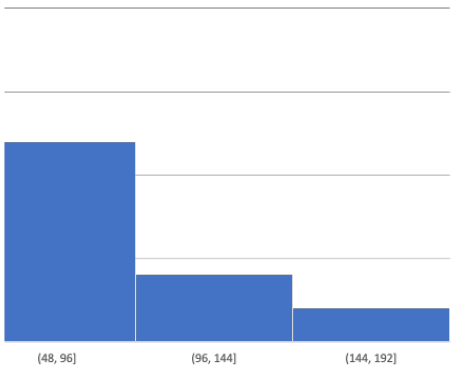
\includegraphics[width=0.5\linewidth]{images/isto.png}
\end{figure}

\subsubsection{Deviazione standard campionaria}
La deviazione standard misura quanto i valori numerici di una caratteristica sono dispersi rispetto alla media.

\noindent Se il grafico ha una forma a campana simmetrica:
\begin{itemize}
    \item $\sigma$ piccola indica valori vicini alla media 
    \item $\sigma$ grande indica valori lontani dalla media, valori dispersi 
\end{itemize}

\begin{figure}[H]
    \centering
    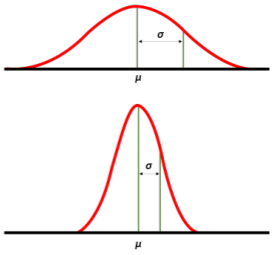
\includegraphics[width=0.5\linewidth]{images/deviazione-standard.png}
\end{figure}

\noindent La formula prevede di calcolare la varianza di ciascun valore (distanza dalla media al quadrato) divisa per il numero di valori, il tutto 
sotto radice.

\subsubsection{Mediana}

La mediana è quel valore che divide l'insieme a metà; è quel valore per cui il 50\% dei valori è più piccolo e l'altro 50\% è più grande.

\subsubsection{Quartili}
\begin{itemize}
    \item \textbf{Primo quartile:} valore $x$ tale che 25\% dei valori è minore di $x$
    \item \textbf{Secondo quartile:} valore $x$ tale che 50\% dei valori è minore di $x$
    \item \textbf{Terzo quartile:} valore $x$ tale che 75\% dei valori è minore di $x$
\end{itemize}

$\Rightarrow$ il secondo quartile coincide con la mediana 

\noindent La \textbf{differenza interquartile} (differenza tra terzo e primo quartile) è utile per fare analisi su dati la cui distribuzione non è 
a campana simmetrica, dato che la deviazione standard ha senso di essere usata solo su dati che seguono quella distribuzione (altrimeniti la 
media non sarebbe un valore tipico, non avrebbe senso misurare la distanza da essa).

\subsection{Relazione tra due feature}

Ci si può chiedere se due colonne di un dataset siano correlate, ovvero se sono legate a tale punto che mi basta saperne una per conoscere anche l'altra.

\noindent Si possono mettere le due caratteristiche su un piano e rappresentarle graficamente per vedere se esiste una correlazione:

\begin{figure}[H]
    \centering
    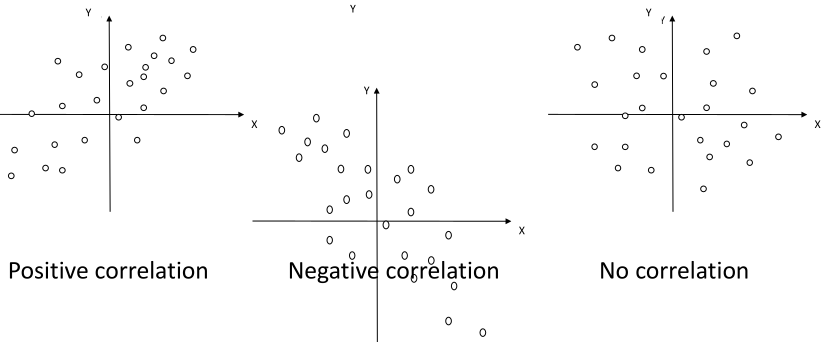
\includegraphics[width=1\linewidth]{images/correlazione.png}
\end{figure}

\noindent È possibile usare due metriche:
\begin{itemize}
    \item \textbf{Varianza:} dà informazioni sulla variabilità interna di una variabile 
    \item \textbf{Covarianza:} dà informazioni su come due variabili variano insieme; mi dice quanto il variare di una 
    influenzi il variare dell'altra
    \begin{itemize}
        \item \textit{Positiva:} le variabile variano nella stessa direzione 
        \item \textit{Negativa:} le varaibili variano nella direzione opposta
        \item \textit{Zero:} nessuna correlazione
    \end{itemize}
\end{itemize}

\noindent La covarianza viene usata per ottenere un numero tra -1 e 1 (tramite il \textit{coefficiente di correlazione di Pearson}) che mi dice quanto due variabili sono correlate tra loro.

\begin{itemize}
    \item due variabili si dicono indipendenti se non condividono informazioni 
    \item se sono dipendenti, la \textit{quantità di informazione} condivisa si stima con la correlazione
\end{itemize}

\noindent Bisogna fare attenzione a fare una distinzione tra correlazione e causa. Potrebbe sembrare che due correlazioni siano 
correlate solo perchè sono correlate ad una terza grandezza; è il caso ad esempio di suicidi e mangiare aringhe.

\subsubsection{Distribuzioni asimmetriche}
Quando un istogramma è costruito su valori che seguono una \textit{distribuzione normale}, allora la forma delle colonne sarà \textit{a campana}; 
tuttavia, in casi reali gli istogrammi sono spesso asimmetrici.

\subsection{Decision Making via algorithms}
\textit{Per quale motivo si cerca di rispondere ad un problema tramite un modello supervisionato? 
Non basterebbe avere un algoritmo?}

\noindent Gli algoritmi applicano una \textbf{teoria} alle grandezze (ad esempio la deteriorità di un motore elettrico dovuta alla temperatura); se ho una 
teoria, la posso \textbf{esplicitare con un algoritmo:} ho una funzione che lega input e output; non ho più bisogno di avere esempi, ma ho la teoria 
che mi dice che la deteriorità del motore è dovuta al numero di ore, ad una determinata temperatura\dots

\noindent Molti problemi non possono essere risolti in questo modo, dato che non c'è un'equazione esplicita; la devo \textit{tirare fuori} dall'addestramento 
del modello.


\subsection{Decision Making via Supervised Machine Learning}
Non viene usata una formula e algoritmo che descrive in modo esplicito un fenomeno per derivare l'informazione per prendere una decisione. Viene 
usata una \textbf{formula generica con dei parametri, che vengono regolati per minimizzare l'errore}. Si tratta dunque di trovare i valori 
giusti dei parametri, viene fatto nella fase di addestramento.

\noindent Viene associato a ciascun valore un peso; alla somma pesata viene poi aggiunta una costante a cui \textit{viene applicato un 
sogliatore}; in questo modo l'output è una funzione non lineare, invece che una semplice somma pesata.

\noindent La procedura di addestramento consiste nel \textbf{considerare l'errore come funzione dei pesi}, andando poi a modificarli per 
minimizzarli.

\noindent Un singolo neurone può approssimare solo una funzione lineare:

\begin{figure}[H]
    \centering
    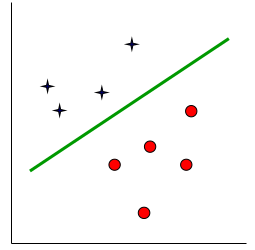
\includegraphics[width=0.4\linewidth]{images/linear.png}
\end{figure}

\noindent Una \textit{rete neurale multi-livello} può teoricamente approssimare qualsiasi funzione dopo 
una certa soglia (\textit{diventa Touring-complete}):

\begin{figure}[H]
    \centering
    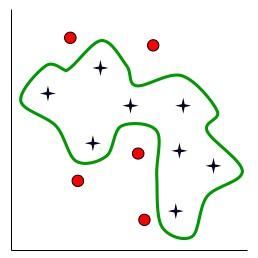
\includegraphics[width=0.4\linewidth]{images/touring-completo.png}
\end{figure}

\subsection{Ciclo di vita di un modello di ML}
L'addestramento è solo una delle parti di vita di un modello di machine learning:
\begin{itemize}
    \item \textbf{Data Management:} costruzione del dataset, controlli di vario tipo, eliminare colonne correlate tra loro \dots
    \item \textbf{Model Learning:} addestramento del modello 
    \item \textbf{Model Tuning:} fase post-addestramento in cui si danno al modello dati che non ha mai visto 
    \item \textbf{Modelo Deployment:} il modello viene messo in produzione nel caso in cui soddisfi i requisiti; altrimenti, viene 
    riportato indietro alle fasi precedenti
    \item \textbf{Model Maintenance:} si può avere un degradamento delle prestazioni perchè cambiano le distribuzioni dei dati in ingresso (è 
    preferibile che siano gaussiane e stazionarie); devo fare gli opportuni controlli 
\end{itemize} 

\noindent Ciascuna di queste fasi può subire un attacco.

\begin{figure}[H]
    \centering
    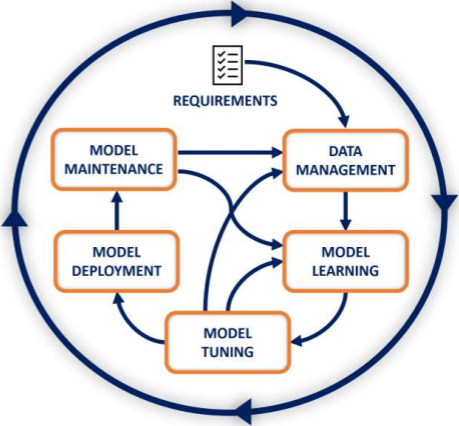
\includegraphics[width=0.6\linewidth]{images/ml-life-cycle.png}
\end{figure}


\section{Introduzione a Machine Learning}

\begin{itemize}
    \item I modelli supervisionati vanno addestrati; sono soggetti ad attacco in fase di inferenza ed in fase di training
    \item I modelli non supervisionati processano i dati sulla base delle loro proprietà, non su esempi che hanno visto; ad esempio, 
    le tecniche di clustering sono basate sulla definizione di distanze intragruppo e intergruppo. Non esiste una 
    fase di training in cui possono essere attaccati
\end{itemize}

\begin{figure}[H]
    \centering
    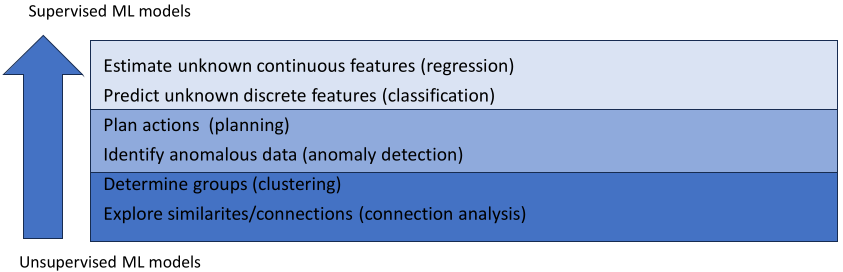
\includegraphics[width=1\linewidth]{images/intro-ml.png}
\end{figure}

\noindent Regressore e classificatore fanno parte delle task di completamento.

\subsection{Paradigma Supervised Learning}
Il problema è \textbf{imparare una relazione tra input e output a partire da degli esempi}; viene prima addestrato il modello e poi se ne ottiene uno (addestrato)
che può essere messo in produzione. In sede di addestramento il modello viene regolato per cercare di \textbf{minimizzare l'errore}.

\noindent Può essere attaccato, per cercare di violare alcune proprietà (accuratezza, ma non solo), posso cercare di fargli sbagliare un input in 
particolare, posso fare violazioni di privacy cercando se un determinato elemento appartiene al training set \dots


\noindent L'idea per creare un modello è:
\begin{itemize}
    \item viene dato un input, e il modello produrrà un output sicuramente sbagliato 
    \item si va a modificare i pesi per cercare di ridurre l'errore 
    \item si continua così fino a che ottengo dei buoni risultati che minimizzano l'errore 
    \item una volta finito questo processo, il modello non ancora pronto, perchè funziona bene sui dati che ha già visto 
    
    $\rightarrow$ devo fare una fase di testing sui dei valori che non ha mai visto (\textit{test set})
\end{itemize}

\subsubsection{\textit{Supervised ML Training in a nutshell}}
\begin{itemize}
    \item Il modello interno più semplice è una somma pesata; si ha un input multivariato, dove ogni variabile viene moltiplicata per un peso per poi
    fare la sommatoria
    \item A questa somma pesata viene poi applicata una soglia (ad esempio, se è sopra la soglia considero il risultato benigno mentre se è sotto 
    considero maligno)
    \item Quando ottengo il risultato, viene confrontato con quello reale (siamo nella fase di training), e se ho fatto un errore si va 
    a modificare i pesi cercando di diminuire l'errore
    \item Si continua tante volte in questo modo sul training set, sperando che l'errore continui a diminuire sempre di più fino a fermarmi 
    nel punto di minimo ($gradiente = 0$, ovvero la derivata delle funzioni multivariate)
\end{itemize}

\noindent All'input viene aggiunta una costante che prende il nome di \textbf{bias}, che aiuta a migliorare l'output riducendo la varianza 
e beneficiando all'accuratezza. Il training \textit{decide la quantità di bias} che massimizza l'accuratezza.

\noindent Mettendo più strati di neuroni (l'output di uno va in input ad un altro) si riesce a fare un addestramento più rapido; con 3 o più strati 
si dice che la rete è \textit{Touring completa}.

\subsubsection{Error backpropagation}
Uno dei problemi della rete neurale tradizonale è quello di non riuscire a fare una corretta \textit{error backpropagation}, ovvero non 
si riesce a distribuire l'errore anche sugli strati interni.

\noindent Per arginare questo problema si usano i primi strati per modificare la rappresentazione degli input, comprimendoli 
in una parte più piccola, mentre sono solamente gli 
ultimi quelle che vengono effettivamente addestrati.

\subsubsection{Overfitting}
Bisogna fare attenzione all'\textit{overfitting}: significa che il modello commette errore pari a 0 sui dati del training set, ma che 
su dati mai visti prima commette un grande errore; questo accade perché il modello non è in grado di generalizzare.

\noindent Per evitare che un modello vada in overfitting, generalmente un il training viene fermato prima di raggiungere un'accuratezza perfetta 
sui dati di training.


\subsection{Diversi modelli di Machine Learning}
\begin{itemize}
    \item \textbf{Classificazione:} mappa vettori di caratteristiche in \textit{categorie} o \textit{classi}
    \item \textbf{Anomaly Detection:} serve a capire se un input è anomalo rispetto a quello atteso 
    \item \textbf{Predizione:} un classificatore può anche agire da predittore, come ad esempio prevedere l'esito di un azione. Per fare il training 
    gli do sole la parte iniziale dei dati e li faccio classificare come successo/insuccesso
    \item \textbf{Planning:} sono adatti in cui non riesco a calcolare l'errore per ogni singolo input; ad esempio, se gioco a scacchi è difficile 
    classificare una singola mossa come buona o cattiva\dots

    $\rightarrow$ si usa un sistema di \textit{reward}, non calcolato sulla singola mossa ma su una sequenza di mosse
    \item \textbf{Connection Analytics:} analizza la relazione tra utenti/sistemi; fondamentale per la sicurezza (ad esempio, individuare 
    nodi centrali o vulnerabili)
\end{itemize}

\noindent $\Rightarrow$ lo stesso problema può essere risolto con modelli diversi; la scelta dipende dai dati disponibili







\chapter{AI-Based Decision Making}

\section{Regressore}

Il regressore è una sorta di \textit{via di mezzo} tra un classificatore e un anomaly detector; utilizza il residuo quadratico 
per restituire valori continui invece che una singola eticheta (data una $x$ che non ha mai visto prima, mi restituisce la sua $y$).

\noindent Fare la regressione significa trovare la retta (o iperpiano) che minimizzi la somma dei quadrati delle distanze dei punti dalla retta.

\begin{figure}[H]
    \centering
    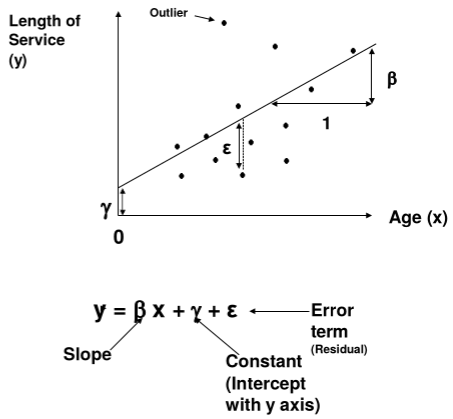
\includegraphics[width=0.6\linewidth]{images/regressore.png}
\end{figure}

\subsubsection{Qualità del regressore}

Se mi accorgo che il regressore restituisce costantemente valori \textit{troppo più alti (o bassi)}, allora significa che l'intercetta con l'asse $x$
del regresspre è posizionata troppo in alto (o in basso) rispetto ai punti futuri. Si dice in questo caso che \textit{sto usando un bias}; si può 
\textit{aggiustare} la retta aggiungendo i nuovi punti o rimuovendo quelli più vecchi.

\subsubsection{Validazione}
Per evitare overfitting e prendere il miglior regressore possibile, si ha bisogno di due set:
\begin{itemize}
    \item \textbf{Training set:} usato per minimizzare l'errore quadratico 
    \item \textbf{Test set:} verifico che errore ho ottenuto e guardo se c'è un bias
\end{itemize}


\subsubsection{Bias-Varianza trade off}
L'errore dipende sia dalla varianza che dal bias; si cerca di minimizzare entrambi, ovvero che sbaglio poco (varianza) e quel poco 
che sbaglio è ben distribuito (bias).

\noindent Purtroppo però quando muovo la retta per minimizzare l'errore, non riesco a minimizzare entrambi: al diminuire di uno cresce l'altro.

\subsection{Regressione Ridge e Lasso}

Sono dei metodi di regressione che introducono dei vincoli sui coefficienti del regressore, portando ad avere un regressore 
più sofisticato; cercano di trovare un compromesso tra varianza (quanto sbaglia) e bias (in che direzione sbaglia).

\subsubsection{Regressione Ridge}
Cerca di limitare la dimensione dei coefficienti, definendo un parametro $\lambda$ pari alla somma dei quadrati dei coefficienti.

\noindent L'obiettivo è cercare di impedire ai punti di training di generare un predittore con un bias troppo alto per aver voluto 
minimizzare l'errore. Inoltre, la tutti i coefficienti devono avere valori diversi da 0, perchè voglio che il regressore prenda in 
considerazione tutte le variabili.

\noindent Il parametro $\lambda$ viene scelto usando un set di validazione: lo scelgo sui dei dati selezionati di cui mi fido, per poi 
usarlo su tutto il training set.

\subsubsection{Regressione Lasso}
È simile alla \textit{ridge regression}, con la differenze che è permesso mettere i valori dei coefficienti pari a 0. La regressione Lasso impone 
che la somma dei valori assoluti dei coefficienti sia minore di un certo valore, portando alcuni coefficienti ad essere pari a 0.

\noindent Questo può portare ad avere dei modelli più semplici che non includono alcune features.

\subsection{Regressore multivariato}

Si passa ad un modello multivariato; l'output (la $y$) dipende da una combinazione lineare degli input.

\noindent Le condizioni per aver un buon regressore multivariato sono che:
\begin{itemize}
    \item gli errori siano indipendenti 
    \item la distribuzione degli errori è gaussiana 
    \item la varianza è costante
\end{itemize}

\noindent Una volta ottenuto un predittore, lo posso usare e sarà molto più rapido di un'inferenza tramite rete neurale.

\subsection{Coefficiente di determinazione multipla}

Rappresenta la spiegabilità del risultato di un regressore, ovvero fornire una descrizione dei fattori che hanno influenzato la decisione.

\noindent Il modo più semplice è fare l'analisi di quali feature hanno influenzato di più la decisione: viene fatto tramite il coefficiente $r^2$
calcolabile nel seguente modo:

\begin{figure}[H]
    \centering
    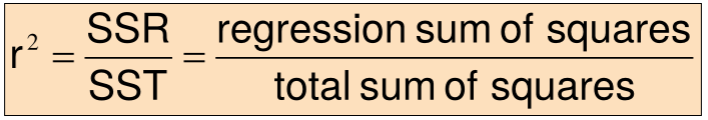
\includegraphics[width=0.6\linewidth]{images/r2.png}
\end{figure}

\noindent Questo coefficiente mi dice quanto è collettiva l'influenza delle variabili: magari ce n'è una che conta tantissimo e un'altra che 
è ininfluente. Mi dice quanto è collettiva la decisione, se dipende da tutte le variabili o se solo da un loro sottoinsieme.

\noindent Esistono test statistici per scartare le variabili che sono poco influenti: se un coefficiente è basso vuol dire che influenza 
poco, lo potrei scartare per avere un regressore più semplice.


\subsection{Interazione tra variabili}
Avviene quando sospetto che l'influenza di una variabile dipende dal valore delle altre: ad esempio, sospetto che l'influenza su $y$
di $x_2$ dipenda dal valore di $x_1$. Si può modellare introducendo i 
\textbf{prodotti incrociati}; è un'interazione tra le variabili di input, si ottiene una combinazione non lineare.

\begin{figure}[H]
    \centering
    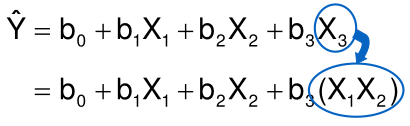
\includegraphics[width=0.6\linewidth]{images/prodotti-incrociati.png}
\end{figure}


\section{Basic ML models}

L'obiettivo di un modello di machine learning è aprossimare una funzione $f$ che non conosciamo. Ciò che cambia è il dominio e codominio:
\begin{itemize}
    \item se il codominio è un set finito di etichette $\Rightarrow$ classificatore 
    \item se il codominio è un numero reale $\Rightarrow$ regressore 
    \item se il codominio è un valore $\Rightarrow$ predittore 
\end{itemize}


\subsection{Alberi di decisione}

Gli alberi di decisione sono un modello di regressione o classificazione sotto forma di albero. L'albero viene costruito dividendo il dataset 
in sottoinsiemi sempre più piccoli, fino ad ottenere un albero composto da:
\begin{itemize}
    \item \textbf{nodi decisionali}
    \begin{itemize}
        \item hanno due o più rami, ciascuno corrispondente a un valore della feature in esame 
    \end{itemize}
    \item \textbf{nodi foglia}
    \begin{itemize}
        \item rappresentano l'esito finale della decisione, cioè la predizione di un valore numerico (nel caso di regressore) o della classe (nel caso 
        di classificatore)
    \end{itemize}
\end{itemize}

\noindent Possono gestire sia dati numerici che categorici.

\begin{figure}[H]
    \centering
    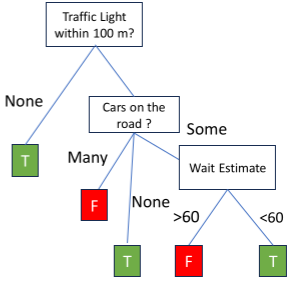
\includegraphics[width=0.6\linewidth]{images/decision-tree.png}
\end{figure}

Un modo per costruire l'albero ed ordinare gli attributi è quella di farlo per \textbf{entropia massima}: dovrei cercare di prendere 
per primo quello con l'entropia più alta. Quando invece faccio la bucketizzazione, dovrei cercare di minimizzare l'entropia.

\subsubsection{Esempio animato}

\begin{figure}[H]
    \centering
    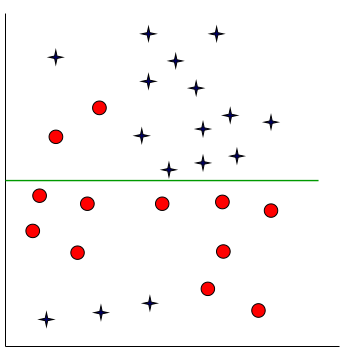
\includegraphics[width=0.4\linewidth]{images/split1.png}
\end{figure}

\noindent Ciasuno dei due insiemi che ho ottenuto sono il più possibile \textit{tutti uguali} $\rightarrow$ ho ridotto l'entropia 

\begin{figure}[H]
    \centering
    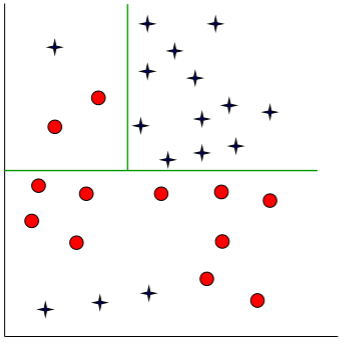
\includegraphics[width=0.4\linewidth]{images/split2.png}
\end{figure}

\begin{figure}[H]
    \centering
    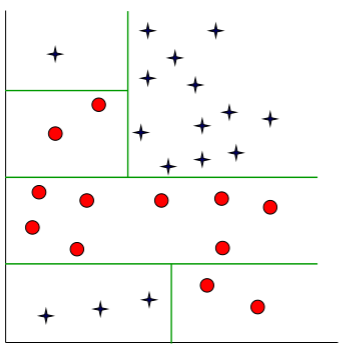
\includegraphics[width=0.4\linewidth]{images/split3.png}
\end{figure}

\noindent Ciascun sottoinsieme ha dati con la stessa etichetta; in questo caso l'albero di decisione fa zero errori sul training set, anche se 
devo stare attento all'overfitting.

\subsection{Nearest Neighbor Models}

Si può dire che il modello è il training set, dato che non devo addestrare niente ma una nuova etichetta viene stimata a partire dal training 
set; quando mi arriva un nuovo punto (ad esempio un dipendente con età e anni di servizio), vado a vedere il punto più vicino a lui nello spazio 
multidimensionale, e uso la sua stessa etichetta.

\noindent Una estensione è quella di usare i $k$ punti più vicini.

\noindent Nell'esempio in figura, il nuovo punto è il quadrato; nel caso a sinistra dirò che è un cerchio, mentre nel caso a destra $(k=3)$ dirò che 
è una croce.

\begin{figure}[H]
    \centering
    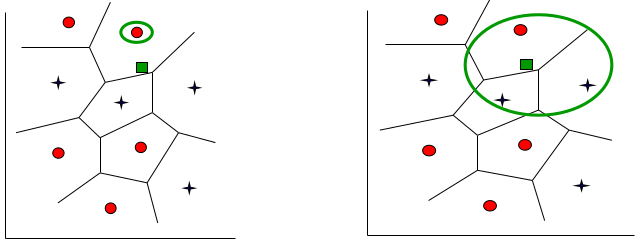
\includegraphics[width=0.8\linewidth]{images/nn.png}
\end{figure}

\subsection{Linear Support Vector Machines}
È un metodo di classificazione in cui prendo il training set e cerco se trovo un iperpiano (nell'esempio una retta) che 
divida in due training set. Vengono calcolati i vettori di supporto (distanze delle coppie rosso-verde con distanza minima) e viene calcolato 
l'iperpiano che li taglia nel modo più ortagonale possibile.

\begin{figure}[H]
    \centering
    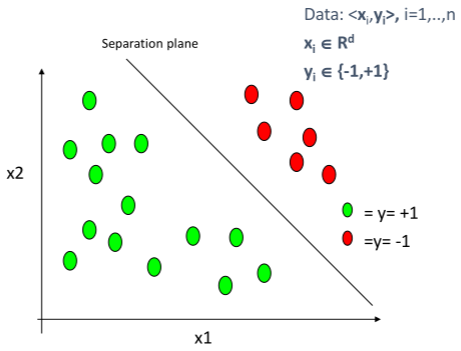
\includegraphics[width=0.6\linewidth]{images/svm.png}
\end{figure}

\noindent I punti di training usati per generare il modello sono relativamente rispetto ad altri modelli, come le reti neurali.

\noindent Dato che non è sempre possibile determinare una separazione netta delle feature, è possibile definire nuove variabili in funzione delle 
altre con funzioni non lineari. Ad esempio, posso usare una funzione non lineare per trasformare le variabili in uno spazio nuovo (ad esempio 
da due a tre dimensioni), dove è più facile calcolare l'iperpiano di seperazione.





\chapter{Gestione dei dati}

\section{Managing Data for AI}

Nel procedimento per passare dai dati grezzi a quelli per il training ci sono tutta una serie di operazioni da fare; assumono particolare importanza quelle di 
\textit{compliance}, tra cui quella più importante è quella per la privacy. Vengono fatte sia per migliorare la qualità del dato che per introddure 
rumore per questioni di privacy.


\noindent Alcune tra le principali fasi di una \textit{data lake}, ovvero una infrastruttura per la gestione di informazioni da dare in pasto 
a modelli di ML, sono:
\begin{itemize}
    \item \textbf{Acquisizione} dei dati 
    \item \textbf{Integrazione} dei dati; ad esempio, se mancano dei dati vado a riempire usando dei dati plausibili (posso prendere 
    un punto vicino per stimare quello che manca), per rendere i miei dati più completi. Viene anche introdotto rumore per questioni 
    di privacy 
    \item \textbf{Storaging}
    \item \textbf{Analytics}
\end{itemize}

\section{Migliorare la qualità dei dati}

\subsection{Ingegneria delle feature}

I modelli neurali di grandi dimensioni riescono a lavorare sui dati grezzi, mentre i modelli semplici (come quelli visti fino ad 
adesso) lavorano su feature che hanno subito un \textbf{processo di analisi}: diminuire la covarianza, togliere feature spurie \dots operazioni 
finalizzati ad ottenere delle features con una \textbf{distribuzione gaussiana}; lavorano su dati con meno dimensioni, le cui dimensioni sono state 
selezionate a mano.

\noindent Se non faccio un processo di \textit{feature engeneering} il training sarà molto più oneroso, mentre se viene fatta il training 
sarà molto più efficacie.

\subsubsection{Alcuni metodi di selezione delle features}

\begin{itemize}
    \item \textbf{Filtraggio:} vengono tolte le features che si possono togliere
    \item \textbf{Wrapping:} viene usato un modello per generare delle coordinate in più da affiancare a quelle originali; data una feature, il modello 
    mi dice una pseudofeature che poi verrà data in pasto al modello semplice.

    $\rightarrow$ Più features vengono \textbf{aggregate} in una pseudofeature, in modo che sarà più semplice da addestrare; il modello da addestrare 
    in questo modo avrà una dimensionalità più bassa del problema
    \item \textbf{Embedding:} vengono scelte solo alcune feature, scartandone altre sulla base dei valori (ad esempio sulla base di valori statistici 
    come la covarianza); è una sorta di filtro dinamico
\end{itemize}

\subsubsection{Filtraggio univariato}
È un metodo di filtraggio usato per filtrare una caratteristica tra poche; non si presta a dei dati \textit{multidimensionali}.

\noindent Il procedimento è il seguente:
\begin{itemize}
    \item calcola la correlazione tra tutte le possibili coppie 
    \item per tutte le coppie la cui correlazione è alta, scarta una delle due caratteristiche in modo casuale 
    \item si ripete il procedimento 
\end{itemize}

\noindent Non è efficiente nel caso feature elevate perchè si devono calcolare tutte le possibili combinazioni.

\subsection{Valori mancanti}

Il modello deve avere colonne con la stessa densità; non ci devono essere colonne troppo vuote o troppo piene rispetto alle altre.

\noindent Nel caso di valori mancanti, si possono modelli come il \textit{k nearest neighbor} per stimarli.




\chapter{Classificazione e Predizione}

\section{Problemi di classificazione}

i modelli di classificazione generalmente sono modelli neurali, dove l'input è una codifica vettoriale e l'output è la classe 
a cui l'input appartiene; durante il training i parametri del modello vengono adattati per ottenere un errore accettabile.

\noindent Tuttavia, per valutare un modello non basta considerare solo l'errore, ma bisogna tenere in considerazione altri fattori come:
\begin{itemize}
    \item dimensione e complessità del classificatore ottenuto 
    \item quantità di dati di training 
\end{itemize}

\subsubsection{Confusion Matrix}

Viene utilizzata per mostrare per ciascuna riga e colonna gli errori nella classificazione:

\begin{figure}[H]
    \centering
    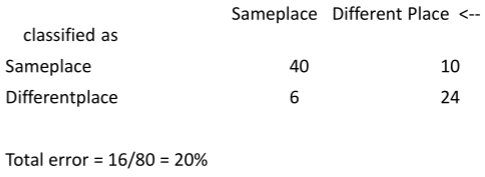
\includegraphics[width=0.7\linewidth]{images/confusion-matrix.png}
\end{figure}


\subsubsection{Curve ROC}

Si ottiene riportando falsi positivi e falsi negativi su un piano (quando si tratta di un classificatore binario). Dove è preferibile posizionarsi 
su questa curva nella fase di training dipende dal contesto e dall'impatto di ciascuno dei due errori (gli errori non hanno tutti lo stesso peso\dots).

\subsubsection{Cross-Validation}

Consiste nel dividere il dataset in un $80\%$ usato per il training, e il restante $20\%$ per fare validation; questo processo viene ripetuto 
più volte fino al raggiungimento di un'accuratezza uniforme. È un modo per \textit{approssimare} la capacità del modello di generalizzare, anche se 
bisogna tenere conto che i punti del validation test sono stati punti del training set in una fase precedente.

\noindent Con la metodologia \textit{held-out} si usa un set mai visto prima per fare validation.


\subsubsection{Precision e Recall}

\textit{Precision} equivale a dire \textit{"quanti sono classificati correttamente tra tutti quelli classificati come X?"}

\begin{figure}[H]
    \centering
    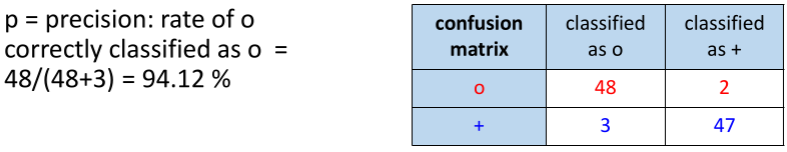
\includegraphics[width=1\linewidth]{images/precision.png}
\end{figure}

\noindent Recall equivale a dire \textit{"tra gli elementi della classe X, quanti sono stati classificati come X?"}

\begin{figure}[H]
    \centering
    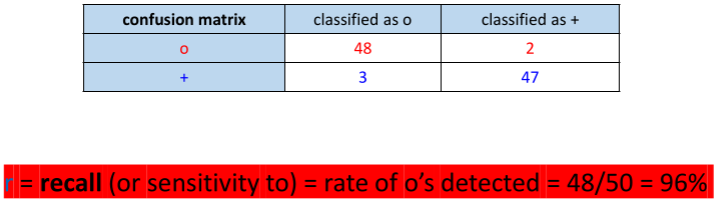
\includegraphics[width=0.9\linewidth]{images/recall.png}
\end{figure}

\noindent $\Rightarrow$ la differenza sta nel chiedersi \textit{classificati correttamente rispetto a cosa? a quelli totali o a quelli della classe?}

\noindent Tipicamente, all'aumentare di una diminuisce l'altra; dato che si è interessati nel massimizzare entrambe le metriche, si può usare 
il parametro \textit{F-score}, che è una sorta di media armonica delle due.

\begin{figure}[H]
    \centering
    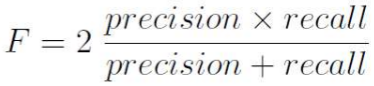
\includegraphics[width=0.4\linewidth]{images/f-score.png}
\end{figure}

\subsubsection{Considerazioni sull'addestramento}

Conoscendo il costo dei diversi tipi di errori, potrei cercare di fare in modo di regolare i parametri per minimizzare il costo totale 
degli errori; bisogna sempre fare attenzione a non andare in overfitting, ovvero quando il modello è troppo adatto al training set e 
non sarà in grado di generalizzare.

\begin{figure}[H]
    \centering
    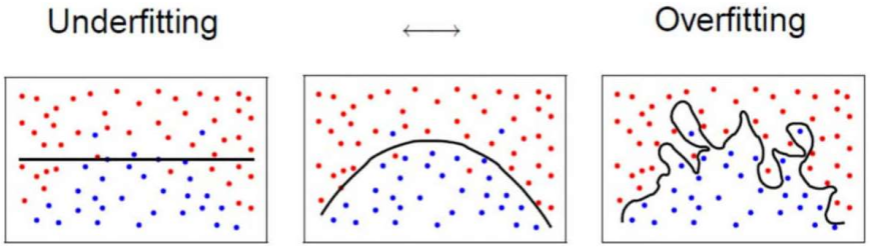
\includegraphics[width=1\linewidth]{images/overfitting.png}
\end{figure}


\section{Deep Classifier Models}

Quando si ha una rete a tanti livelli si ha il problema di dove ripartire l'errore sui vari pesi.

\noindent Un possibile approccio potrebbe essere quello del \textbf{training strato per strato:} vengono \textit{bloccati} tutti gli strati 
tranne uno (nel senso che non vengono modificati i parametri), per poi pertubrare i pesi dello strato non bloccato nelle varie direzioni, scegliendo 
quella in cui l'errore diminuisce maggiormente. 

\noindent Questo procedimento viene ripetuto più volte passando strato per strato, fino ad ottenere un modello che ha per parametri i vari pesi 
che sono stati addestrati separatamente; ovviamente, il procedimento deve essere ripetuto più volte, perchè magari quando modifico i parametri 
per uno strato sto generando errore \textit{da un'altra parte}.

\noindent Questo metodo funziona discretamente con reti \textit{shallow}, ovvero con pochi strati.

\noindent A metà anni 2000 è stato introdotto una nuova metodologia: consiste nel non fare training di tutti gli strati, ma di 
fare usare il training set con le label per addestrare solo gli ultimi due strati della rete; gli strati precedenti sono utilizzati per 
la \textbf{costruzione di uno spazio latente}. In altre parole, il loro scopo è \textbf{trovare un encoding dei punti di input che mantenga la 
loro correlazione statistica ma su un numero diverso di features}; non mira quindi a prevedere la label.

\noindent Qualunque sia la distribuzione di ingresso (si spera Gaussiana su più variabili), si va a cercare un encoding su meno features tale che 
sia anch'esso multivariato Gaussiano, e che la divergenza (la distanza tra le due distribuzioni) sia pari a 0: questo è ciò in cui consiste il 
training di tutti gli strati intermedi. 

\noindent L'idea è che le features che escono (che sono meno) sono quelle su cui poi si addestrano gli ultimi strati.

\begin{figure}[H]
    \centering
    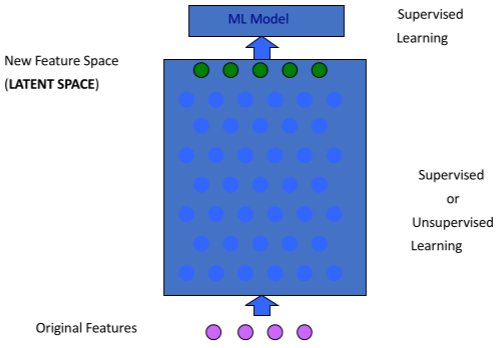
\includegraphics[width=0.6\linewidth]{images/spazio-latente.png}
\end{figure}

\noindent Nella figura lo spazio latente è inflattivo, ovvero escono più features di quelle che sono entrate. Non deve essere per forza così, può 
essere anche deflattivo a seconda dei casi.


\noindent $\Rightarrow$ il deep learning consiste in:
\begin{enumerate}
    \item fase di pre-training degli strati iniziali (auto-encorders)
    \begin{itemize}
        \item questa fase è non-supervisionata perchè non mi interessa delle etichette di classificazione, mi interessano solo le distribuzioni dei 
        punti per calcolare la divergenza (sono parametri estraibili dal training set)
    \end{itemize}
    \item fase di training supervisionato sugli strati finali; è la classica classificazione con minimizzazione dell'errore 
\end{enumerate}

\subsubsection{\textit{Unsupervised Pre-Training in a nutshell}}

Supponiamo di avere una rete di un solo strato con $n$ input ed output, e $k$ parametri intermedi con $k<n$

\noindent Viene fatto un training di \textit{riproduzione esatta}, ovvero si addestra lo strato e riprodurre esattamente gli input; una volta 
addestrato il modello, si rimuove il layer di output.


\subsubsection{Layer convoluzionale}

Una rete neurale convoluzionale è una rete neurale con alcuni strati convoluzionali: ciò che fanno è sommare dei gruppi di input per 
ottenere un layer a covarianza ridotta rispetto al layer originale.

\noindent Gli input sono collegati a dei filtri, e l'output del filtro (che è una sorta di somma pesata) è collegato al layer successivo. Si usano 
questi raggruppamenti di input come se fossero un encoder, ovvero si usano per ottenre in output un'altra rappresentazione dell'input.

\begin{figure}[H]
    \centering
    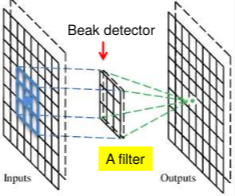
\includegraphics[width=0.5\linewidth]{images/convolutional.png}
\end{figure}

\noindent Si usa una rete convoluzionale per eseguire un encoding; tuttavia, un encoding non è necessariamente convoluzionale.


\section{Autoencoders}

È un tipo di apprendimento non-supervisionato che trasforma l'\textit{input raw} in \textit{input latente}.

\begin{figure}[H]
    \centering
    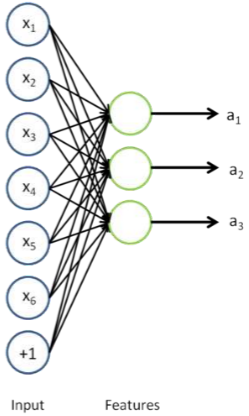
\includegraphics[width=0.5\linewidth]{images/autoencoder.png}
\end{figure}


\noindent Si può che impara delle feature generiche dai dati di input, 
estraendo delle \textit{macrofeatures}.

\noindent Possiamo fare una distinzione tra due tipi di encoder:
\begin{itemize}
    \item \textbf{Deflattivi}, il cui scopo è comprimere l'input
    \item \textbf{Inflattivi}, il cui scopo è il aggiungere rumore ai dati di input 
\end{itemize}


\subsection{GAN - Generative Adversial Network}

Sono modelli deep in grado di produrre dei sample X simili ai dati di input. 

\noindent Si usa un \textbf{discriminatore} per valutare la qualità del dato generato da una GAN: restituisce 1 se lo considero vero, oppure 
0 se lo riconosce come dato che è stato generato; avrò ottenuto un buon generatore quando sarà in grado di ingannare il discriminatore.



\section{Modelli predittivi}

Le serie temporali (dataset in cui una colonna è un timestamp) stanno alla base per poter fare un modello predittivo; consistono in dati 
misurati ad un tempo specifico, generalmente con intervalli regolari. L'analisi delle serie temporali cerca di \textbf{identificare fattori}
che sono influenti sui valori della serie.

\noindent Una serie temportale si dice stazionaria se:
\begin{itemize}
    \item la covarianza tra due punti è indipendente dal momento in cui sono stati osservati 
    \item la media è costante nel tempo 
\end{itemize}

\noindent Le serie stazionarie hanno i migliori predittori lineari, mentre per quelle non stazionarie risulta più complesso e lento implementare 
un predittore.

\subsection{Trend}

Il trend rappresenta l'andamento generale di una serie temporale su un arco di tempo sufficientemente lungo; è rilevabile con i dati disponibili 
solo se l'arco di tempo è abbastanza lungo da permetterlo. Una serie temporale può essere suddivisa in quattro componenti.

\subsubsection{Trend secolare}
Rappresenta l'andamento generale della serie nel lungo periodo; una volta individuato, permette di identificare le altre componenti più facilmente.

\begin{figure}[H]
    \centering
    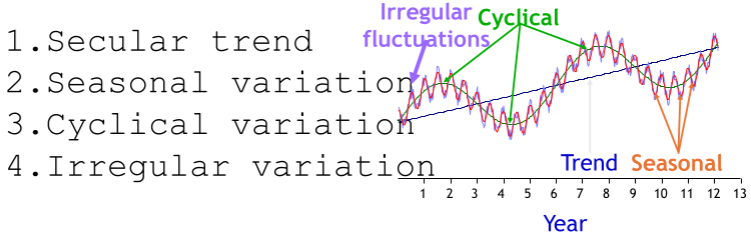
\includegraphics[width=0.7\linewidth]{images/trend.png}
\end{figure}

\subsubsection{Variazione stagionale}
È un pattern di cambiamenti che avviene ad intervallo di tempo regolari; sono spessi legati alle stagioni o ad eventi e festività, come ad esempio 
i casi di influenza in inverno.

\subsubsection{Variazioni cicliche}
Sono dei pattern che si ripetono ma con un intervallo di tempo \textit{più irregolare} rispetto alle variazioni stagionali. Sono più complicati 
da individuare, ed è difficile prevedere per quanto si potrae il periodo di espansione o contrazione.


\begin{figure}[H]
    \centering
    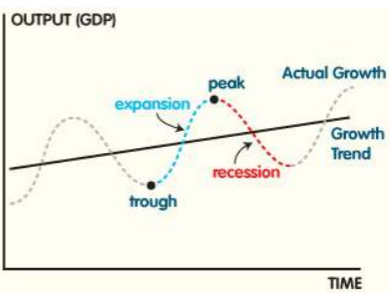
\includegraphics[width=0.6\linewidth]{images/variazioni-cicliche.png}
\end{figure}


\subsubsection{Variazioni irregolari}

Sono delle variazioni casuali nella serie temporale, che non posso essere spiegate con i casi precedenti, come ad esempio dei crolli finanziari 
o catastrofi naturali.

\subsection{Analisi dei trend}

I trend passati stanno alla base per la predizione futura.

\subsubsection{Semi-averages}
Bisogna controllare prima che non ci siano outliers nei dati; la procedura è la seguente:
\begin{enumerate}
    \item dividere i dati in due intervalli di tempo uguali 
    \item calcolare la media per ogni intervallo 
    \item tracciare una retta tra i due punti medi 
    \item estendere la retta nel futuro per fare previsioni 
\end{enumerate}


\subsubsection{Medie mobili}
L'idea è che se la medie è calcolata su intervallo di tempo sufficientemente lungo, l'effetto delle variazioni a breve termine sarà ridotto; in 
altre parole, le variazioni cicliche e stagionali saranno \textit{smussate}, ottenendo un grafico più \textit{morbido} che rappresenta 
il trend generale. 

\noindent Il grado di smussamento può essere regolato selezionando quali valori includere nella media.



















\end{document}
